\documentclass{ximera}

\newcommand{\RR}{\mathbb R}
\renewcommand{\d}{\,d}
\newcommand{\dd}[2][]{\frac{d #1}{d #2}}
\renewcommand{\l}{\ell}
\newcommand{\ddx}{\frac{d}{dx}}
\newcommand{\dfn}{\textbf}
\newcommand{\eval}[1]{\bigg[ #1 \bigg]}


\outcome{Compute surface area using double integrals.}

\title[Dig-In:]{Surface area}

\begin{document}
\begin{abstract}
  We compute surface area with double integrals.
\end{abstract}
\maketitle


In the past, we've used definite integrals to compute the arc length
of curves.  The natural extension of the concept of \textit{arc length
  over an interval} is \textit{surface area over a region.}  Consider
the surface $z=F(x,y)$ over some region in the $(x,y)$-plane. To
compute the surface area, first consider the surface area of a
``patch'' of the surface, determined by $\vec{u}$ and $\vec{v}$ below:
\begin{image}
  \begin{tikzpicture}
    \begin{axis}%
      [width=175pt,height=200pt,
        tick label style={font=\scriptsize},%axis on top,
	axis lines=center,
	view={110}{25},
	name=myplot,
	xtick=\empty,
	ytick=\empty,
	ztick=\empty,
	minor xtick=1,
	minor ytick=1,
	ymin=0,ymax=.5,
	xmin=.6,xmax=1.2,
	zmin=1, zmax=2.1,
        every axis x label/.style={at={(axis cs: .15,-.34,0)}},%,xshift=-1pt,yshift=-1pt},
	xlabel={\scriptsize $x$},
	every axis y label/.style={at={(axis cs:-.5,.2,0)}},%,xshift=1pt,yshift=-1pt},
	ylabel={\scriptsize $y$},
	every axis z label/.style={at={(axis cs:0,-.19,1.6)}},
	zlabel={\scriptsize $z$},
        colormap/cool
      ]      
      \addplot3[domain=0:1.4,,y domain=0:.4,mesh,samples=15,samples y=9,very thin,z buffer=sort] {-.5*(x-1)^2-.5*(y)^2+2};
      
      %\addplot3[draw=mapped color!0!black,,domain=.8:1,surf,y domain=.2:.3,samples=2,samples y=2, very thick,z buffer=sort] {1.96375+.1*(x-.9)-.25*(y-.25)};
      \addplot3[surf,faceted color=black,,domain=.8:1,y domain=.2:.3,samples=2,samples y=2, ultra thick,z buffer=sort] {1.96375+.1*(x-.9)-.25*(y-.25)};
      
      
      \draw [penColor,very thick] (axis cs: .8,.2,1) -- (axis cs: .8,.3,1) -- node [pos=.5,right,black] {\scriptsize $\d x$} (axis cs: 1,.3,1) --node [pos=.5,below,black] {\scriptsize $\d y$}(axis cs: 1,.2,1) --(axis cs: .8,.2,1)--(axis cs: .8,.3,1);

      \draw (axis cs: .9,.33,1.95) node {\scriptsize $\vec u$}
      (axis cs: 1.1,.27,2) node {\scriptsize $\vec v$};
      
    \end{axis}
\end{tikzpicture}
\end{image}
In essence, we zoom in on this portion of the surface to the extent
that the tangent plane approximates the function so well that in this
figure, it is virtually indistinguishable from the surface itself.
Therefore we can approximate the surface area $\d S$ of a ``patch'' of
this region of the surface with the area of the parallelogram spanned
by $\vec{u}$ and $\vec{v}$. Here
\begin{align*}
  \vec{u} &= \vector{\d x,0,\pp[F]{x}\d x}\\
  \vec{v} &= \vector{0,\d y,\pp[F]{y}\d y},
\end{align*}
hence
\begin{align*}
  \d S &= |\vec u\cross \vec v|\\
  &= \left|\vector{\d x,0,\pp[F]{x}\d x}\cross\vector{0,\d y,\pp[F]{y}\d y}\right|\\
  &=\sqrt{1+F^{(1,0)}(x,y)^2+F^{(0,1)}(x,y)^2}\d x\d y.
\end{align*}
Summing these ``patches'' together leads to a double integral.

\begin{definition}\index{surface area}
  Let $z=F(x,y)$ where $\pp[F]{x}$ and $\pp[F]{y}$ are continuous over
  a closed, bounded region $R$. The surface area $S$ over $R$
  is
  \begin{align*}
    S &= \iint_R \d S\\
    &=\iint_R \sqrt{1+F^{(1,0)}(x,y)^2+F^{(0,1)}(x,y)^2}\d A.
  \end{align*}
\end{definition}


\begin{question}
  A table of gradient vectors for a function $F:\R^2\to\R$ is
  given below:
  \begin{image}
    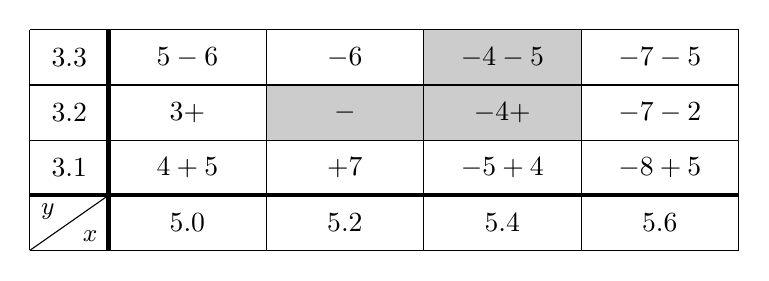
\begin{tikzpicture}[x=1cm,y=.7cm]
      
      \draw[fill=white!80!black] (3,2) -- (7,2) --(7,4) -- (5,4) -- (5,3) -- (3,3)--cycle;
      
      \draw (0,0) grid [step=1] (1,4);
      \draw (3,4) -- (3,0);
      \draw (5,4) -- (5,0);
      \draw (7,4) -- (7,0);
      \draw (9,4) -- (9,0);
      
      \draw (0,0) -- (9,0);
      \draw (0,1) -- (9,1);
      \draw (0,2) -- (9,2);
      \draw (0,3) -- (9,3);
      \draw (0,4) -- (9,4);


  
  \draw[ultra thick] (0,1)--(9,1);
  \draw[ultra thick] (1,4)--(1,0);
  
  \draw (0,0) -- (1,1);
  %\node at (.9,.9) [below left,inner sep=1pt] {\small$y$};
  %\node at (0.1,.1) [above right,inner sep=1pt] {\small$x$};
  \node at (.1,.9) [below right,inner sep=1pt] {\small$y$};
  \node at (0.9,.1) [above left,inner sep=1pt] {\small$x$};
  
  
  %% x-values
  \node at (2,.5) {$5.0$};
  \node at (4,.5) {$5.2$};
  \node at (6,.5) {$5.4$};
  \node at (8,.5) {$5.6$};
  
  %% y-values
  \node at (0.5,1.5) {$3.1$};
  \node at (0.5,2.5) {$3.2$};
  \node at (0.5,3.5) {$3.3$};
  
  
  %% vectors
  %% bottom row
  \node at (2,1.5) {$4\veci+5\vecj$};
  \node at (4,1.5) {$\veci+7\vecj$};
  \node at (6,1.5) {$-5\veci+4\vecj$};
  \node at (8,1.5) {$-8\veci+5\vecj$};
    
  %% second row
  \node at (2,2.5) {$3\veci+\vecj$};
  \node at (4,2.5) {$\veci-\vecj$};
  \node at (6,2.5) {$-4\veci+\vecj$};
  \node at (8,2.5) {$-7\veci-2\vecj$};
  
  %% third row
  \node at (2,3.5) {$5\veci-6\vecj$};
  \node at (4,3.5) {$\veci-6\vecj$};
  \node at (6,3.5) {$-4\veci-5\vecj$};
  \node at (8,3.5) {$-7\veci-5\vecj$};
  
\end{tikzpicture}
\end{image}
Let $R$ be the shaded region above. Estimate the surface area of $F$
over $R$.
\begin{prompt}
  \[
  \text{Area} = \answer{.02\sqrt{3}+.02\sqrt{18}+.02\sqrt{42}}
  \]
\end{prompt}
\begin{hint}
  Use the fact that
  \[
  \d S = \sqrt{1+F^{(1,0)}(x,y)^2+F^{(0,1)}(x,y)^2}\d x \d y
  \]
\end{hint}
\end{question}

\begin{remark}
  In our discussion above, we are in fact \textit{defining} the
  concept of the ``area of a surface.'' While we already have a notion
  of the area of a region in the \textit{plane}, we did not yet have a
  solid grasp of what ``the area of a surface in \textit{space}''
  means. Double integrals make this notion of surface area precise.
\end{remark}

Let's train ourselves to use our new tools by computing the surface
areas of known surfaces. We start with a triangle.

\begin{example}
  Let $F(x,y) = 4-x-2y$, and let $R$ be the region in the $(x,y)$-plane
  \[
  R = \{(x,y):0\le x\le 4\text{ and } 0\le y\le 2-x/2\}
  \]
  \begin{image}
    \begin{tikzpicture}
      \begin{axis}%
        [tick label style={font=\scriptsize},%axis on top,
          axis lines=center,
	  view={125}{25},
	  name=myplot,
	  %xtick=\empty,
	  %ytick={5},
	  %ztick={.7,-.7},
	  minor xtick=1,
	  minor ytick=1,
	  ymin=-.5,ymax=4.5,
	  xmin=-.5,xmax=4.5,
	  zmin=-.5, zmax=4.5,
	  every axis x label/.style={at={(axis cs:\pgfkeysvalueof{/pgfplots/xmax},0,0)},xshift=-1pt,yshift=-4pt},
	  xlabel={\scriptsize $x$},
	  every axis y label/.style={at={(axis cs:0,\pgfkeysvalueof{/pgfplots/ymax},0)},xshift=5pt,yshift=-3pt},
	  ylabel={\scriptsize $y$},
	  every axis z label/.style={at={(axis cs:0,0,\pgfkeysvalueof{/pgfplots/zmax})},xshift=0pt,yshift=4pt},
	  zlabel={\scriptsize $z$},
          colormap/cool
        ]
        \draw [dashed, ultra thick,penColor] (axis cs: 0,0,0) -- (axis cs: 4,0,0) -- (axis cs: 0,2,0) -- cycle;
        %\addplot3[domain=-.1:4.1,,y domain=-0.1:2.1,mesh, very thin,z buffer=sort] {4-x-2*y};
        
        \draw [thick,penColor] (axis cs: 0,0,4) -- (axis cs: 4,0,0) -- (axis cs: 0,2,0) -- cycle;
        
        %\draw [penColor2] (axis cs:0,0,4) -- (axis cs: .8,1.6,0);
      \end{axis}
    \end{tikzpicture}
  \end{image}
  Find the surface area of $F$ over $R$.
  \begin{explanation}
    We start by noting that
    \begin{align*}
      \pp[F]{x} = \answer[given]{-1},\\
      \pp[F]{y} = \answer[given]{-2}.
    \end{align*}
Therefore, from our definition above,
    \begin{align*}
      S &= \iint_R\d S \\
      &= \int_0^{\answer[given]{4}}\int_0^{\answer[given]{2-x/2}} \sqrt{1+(-1)^2+(-2)^2}\d y\d x\\
      &= \int_0^{\answer[given]{4}} \answer[given]{\sqrt{6}\left(2-\frac{x}{2}\right)}\d x\\
      &= \answer[given]{4\sqrt{6}}.
    \end{align*}
    Because the surface is a triangle, we can figure out the area
    using the cross product. Setting
    \begin{align*}
      \vec{v} = \vector{-4,0,\answer[given]{4}},\\
      \vec{w} = \vector{0,-2,\answer[given]{4}},
    \end{align*}
    we see that
    \[
    \vec{v} \cross \vec{w} = \vector{\answer[given]{8},\answer[given]{16},\answer[given]{8}},
    \]
    and so
    \[
    |\vec{v}\cross\vec{w}| = \answer[given]{8\sqrt{6}}.
    \]
    Since this is the area of the parallelogram spanned by $\vec{v}$
    and $\vec{w}$, we divide by $\answer[given]{2}$ to confirm the area of the
    triangle is $4\sqrt{6}$.
  \end{explanation}
\end{example}

    
It's common knowledge that the surface area of a sphere of radius $a$
is $4\pi a^2$. While there are several ways to confirm this formula, we
will use a double integral. Our computation will involves using our
formula for surface area, polar coordinates, and improper integrals!

\begin{example}
Find the surface area of the sphere with radius $a$ centered at the
origin.
\begin{explanation}
  To start, we will compute the surface area of
  \[
  F(x,y) =\sqrt{a^2-x^2-y^2}
  \]
  over the region
  \[
  R = \{(x,y): x^2 + y^2 \le a^2\}.
  \]
  We start by computing partial derivatives and find
  \begin{align*}
    \pp[F]{x} &= \answer[given]{\frac{-x}{\sqrt{a^2-x^2-y^2}}} \\
    \pp[F]{y} &= \answer[given]{\frac{-y}{\sqrt{a^2-x^2-y^2}}}.
  \end{align*}
  Since  our function $F$ only defines the top upper hemisphere of the
  sphere, we double our surface area result to get the total area:
  \begin{align*}
    S &= 2\iint_R \d S \\
    S &= 2\iint_R \sqrt{1+ F^{(1,0)}(x,y)^2+F^{(0,1)}(x,y)^2}\d A \\
    &= 2\iint_R \sqrt{1+ \frac{x^2+y^2}{a^2-x^2-y^2}}\d A.
  \end{align*}
Since the region $R$ that we are integrating over is the circle, we
are likely to have greater success with our integration by converting
to polar coordinates. Using the substitutions
\begin{align*}
  x&=\answer[given]{r\cos(\theta)},\\
  y&=\answer[given]{r\sin(\theta)},\\
  \d A &= r\d r\d \theta,
\end{align*}
we write
\begin{align*}
  S &= 2\iint_R \sqrt{1+ \frac{x^2+y^2}{a^2-x^2-y^2}}\d A\\
  &=2\int_0^{2\pi}\int_0^a \sqrt{1+\frac{r^2\cos^2\theta+r^2\sin^2\theta}{a^2-r^2\cos^2\theta-r^2\sin^2\theta}} r\d r\d\theta
\end{align*}
Simplifying, we now write:
\[
S = 2\int_0^{2\pi}\int_0^a \sqrt{\frac{a^2}{a^2-r^2}} r \d r \d \theta
\]
We evaluate this integral by making the substitution
\begin{align*}
g &= a^2 -r^2,\\
\d g &= \answer[given]{-2r}\d r,\\
\d r &= \frac{\d g}{\answer[given]{-2 r}},
\end{align*}
and paying close attention to the limits of integration, we now have
\[
S = 2\int_0^{2\pi}\int_{a^2}^0\frac{a g^{-1/2}}{-2} \d g \d \theta
\]
However, since the integrand of the inner integral is not defined at
$g= 0$, the inner integral is in fact an improper integral. Let's
carefully evaluate the inner integral. Write with me:
\begin{align*}
  \int_{a^2}^0\frac{a g^{-1/2}}{-2} \d g &= \lim_{b\to 0}\int_{a^2}^b\frac{a g^{-1/2}}{-2} \d g\\
  &= \lim_{b\to 0}\eval{\answer[given]{-a \sqrt{g}}}_{a^2}^b\\
  &= \lim_{b\to 0}(-a \sqrt{b}+ a \sqrt{a^2})\\
  &= \answer[given]{a^2}.
\end{align*}
So we may now write
\begin{align*}
  S &= 2\int_0^{2\pi}\int_{a^2}^0\frac{a g^{-1/2}}{-2} \d g \d \theta\\
  &= 2\int_0^{2\pi} \answer[given]{a^2} \d \theta\\
  &= \answer[given]{4\pi a^2}.
\end{align*}
Thus confirming our previous formula.
\end{explanation}
\end{example}


Let's find the surface area of a general region now.

\begin{example}
  Find the area of the surface $F(x,y) = x^2-3y+3$ over the region
  \[
  R = \{(x,y):-x\le y\le x\text{ and } 0\le x\le 4\}
  \]
  \begin{image}
    \begin{tikzpicture}
      \begin{axis}%
        [width=175pt,height=200pt,
          tick label style={font=\scriptsize},%axis on top,
	  axis lines=center,
	  view={135}{55},
	  name=myplot,
	  %xtick=\empty,
	  %ytick=\empty,
	  %ztick=\empty,
	  %extra x ticks={1},
	  %extra x tick labels={$a$},
	  %extra y ticks={1},
	  %extra y tick labels={$a$},
	  %extra z ticks={1},
	  %extra z tick labels={$h$},
	  ymin=-4.5,ymax=4.5,
	  xmin=-.1,xmax=4.5,
	  zmin=-5, zmax=32,
	  every axis x label/.style={at={(axis cs:\pgfkeysvalueof{/pgfplots/xmax},0,0)},xshift=-1pt,yshift=-4pt},
	  xlabel={\scriptsize $x$},
	  every axis y label/.style={at={(axis cs:0,\pgfkeysvalueof{/pgfplots/ymax},0)},xshift=5pt,yshift=-3pt},
	  ylabel={\scriptsize $y$},
	  every axis z label/.style={at={(axis cs:0,0,\pgfkeysvalueof{/pgfplots/zmax})},xshift=0pt,yshift=4pt},
	  zlabel={\scriptsize $z$},colormap/cool
	]

        \draw [dashed, ultra thick,penColor] (axis cs: 0,0,0) -- (axis cs: 4,4,0) -- (axis cs: 4,-4,0) -- cycle;
       
\addplot3[domain=0:4.5,,y domain=-4.5:4.5,mesh,samples=15,samples y=15,very thin,z buffer=sort] {x^2-3*y+3};

\addplot3[domain=0:4,%fill=white,
penColor,very thick,samples=20,samples y=0] (x,{-x},{x^2+3*x+3});

\addplot3[domain=0:4,%fill=white,
penColor,very thick,samples=20,samples y=0] (x,{x},{x^2-3*x+3});

\addplot3[domain=-4:4,%fill=white,
penColor,very thick,samples=20,samples y=0] (4,{x},{16-3*x+3});

\end{axis}


\end{tikzpicture}
\end{image}


  %% \mfigure[scale=1.2,trim=1mm 0mm 1mm 0mm,
  %% clip]{.3}{Graphing the surface in Example
  %% \ref{ex_surfacearea4}.}{fig:surfacearea4}{figures/figsurfacearea4} }

    \begin{explanation}
      To start, compute the partial derivatives:
      \begin{align*}
        \pp[F]{x} &= \answer[given]{2x}\\
        \pp[F]{y} &= \answer[given]{-3}
      \end{align*}
      Thus the surface area is described by the double integral
      \[
      \iint_R \sqrt{10+4x^2}\d A.
      \]
      As with integrals describing arc length, double integrals
      describing surface area are in general hard to evaluate directly
      because of the square-root. This particular integral can be
      easily evaluated, though, with judicious choice of our order of
      integration.  Integrating with order $\d x\d y$ requires us to
      evaluate
      \[
      \int \sqrt{10+4x^2}\d x.
      \]
      This is not too easy. The computation involves integration by
      parts and $\sinh^{-1}(x)$.

      However, integrating in the order $\d y\d x$ has as its first
      integral
      \[
      \int \sqrt{10+4x^2}\d y,
      \]
      and this is easy to evaluate,
      \[
      \int \sqrt{10+4x^2}\d y = \answer[given]{y\sqrt{10+4x^2}}+C.
      \]
      So we proceed with the order $\d y\d x$. In this case, the
      limits of integration are already given in the statement of the
      problem. Write with me:
      \begin{align*}
        \iint_R\sqrt{10+4x^2}\d A &= \int_0^4\int_{-x}^x\sqrt{10+4x^2}\d y \d x\\
	&= \int_0^4\eval{y\sqrt{10+4x^2}}_{-x}^x \d x\\
	&=\int_0^4\big(2x\sqrt{10+4x^2}\big)\d x
      \end{align*}
      Setting, $g=10+4x^2$ you can use substitution to find:
      \begin{align*}
      \int_0^4\big(2x\sqrt{10+4x^2}\big)\d x &= \eval{\answer[given]{\frac{1}{6}\big(10+4x^2\big)^{3/2}}}_0^4 \\
	&= \frac{1}{3}\big(37\sqrt{74}-5\sqrt{10}\big)
\end{align*}
    Note that the surface has a much greater area than the region in
    the $(x,y)$-plane. This is because the $z$-values of the surface
    change dramatically over $R$.
    \end{explanation}
\end{example}

        
In practice, technology helps greatly in the evaluation of such
integrals. High powered computer algebra systems can compute integrals
that are difficult, or at least time consuming, by hand, and can at
the least produce very accurate approximations with numerical
methods. In general, just knowing \textit{how} to set up the proper
integrals brings one very close to being able to compute the needed
value. Most of the work is actually done in just describing the region
$R$ in terms of polar or rectangular coordinates. Once this is done,
technology can usually provide a good answer.







\end{document}
